\documentclass[11pt]{article}

\usepackage{a4wide}
\usepackage[utf8]{inputenc}
\usepackage[russian]{babel}
\usepackage{graphicx}
\usepackage{amsmath}
\usepackage{amsfonts}
\usepackage{amssymb}
\usepackage{subcaption}
\usepackage{dsfont}
\begin{document}
	
	\thispagestyle{empty}
	
	\begin{center}
		\ \vspace{-3cm}
		
		\includegraphics[width=0.5\textwidth]{msu.eps}\\
		{\scshape Московский государственный университет имени М.~В.~Ломоносова}\\
		Факультет вычислительной математики и кибернетики\\
		Кафедра системного анализа
		
		\vfill
		
		{\LARGE Отчёт по  практикуму:}
		
		\vspace{1cm}
		
		{\Huge\bfseries <<Задача быстродействия>>}
	\end{center}
	
	\vspace{1cm}
	
	\begin{flushright}
		\large
		\textit{Студент 315 группы}\\
		А.\,В.~Бабаев
		
		\vspace{5mm}
		
		\textit{Руководитель практикума}\\
		к.ф.-м.н., доцент П.\,А.~Точилин
	\end{flushright}
	
	\vfill
	
	\begin{center}
		Москва, 2021
	\end{center}
	
	\newpage
	\tableofcontents
	\newpage
	
	{\vspace*{-2cm} \hspace*{-1cm}\section{Постановка задачи и определение параметров}}

	{\hspace{-0.1cm} Задана линейная система обыкновенных дифференциальных уравнений:}
	\newline
	{\[\dot{x} = Ax + Bu + f,\  t \in[t_{0}, +\infty). \]}
	{\hspace{-0.3cm} Здесь $x,f \in \mathbb{R}^{2}, A \in \mathbb{R}^{2 \times 2},  B \in \mathbb{R}^{2 \times 2}, u \in \mathbb{R}^{2}$. На значения управляющих параметров $u$ наложено ограничение: $u \in \mathcal{P}.$ Пусть $\mathcal{X}_{0} - $ начальное множество значений фазового вектора, $\mathcal{X}_{1} - $ целевое множество значений фазового вектора. Необходимо решить задачу быстродействия, т.е. найти минимальное время $T > 0$, за которое траектория системы, выпущенная в момент времени $t_{0}$ из некоторой точки множества $\mathcal{X}_{0}$, может попасть в некоторую точку множества $\mathcal{X}_{1}$.}
	\newline 
	\[\mathcal{P} = \bigg{\{ } (x,y): \ \ \begin{matrix}
	\gamma (x - p_{1})^2 + \alpha (y - p_{2})^2 \leq 1 \quad, \ $при$ \ y \geq p_{2} \\
	\gamma (x - p_{1})^2 + \beta (y - p_{2})^2 \leq 1 \quad, \  $при$ \  y \leq p_{2}
	 	\end{matrix} \bigg{ \} }, \ \ \ \alpha > 0, \ \beta > 0, \ \gamma > 0, \]
	\[ \mathcal{X}_{0} = conv\{q_{1}, q_{2}, q_{3}\} + S_{r}(0) ;  \]	
	\[\mathcal{X}_{1} = \{ x_{1}\}.\]
	\newline
	{\hspace*{-0.3cm} 1)Необходимо написать в среде MatLab программу с пользовательским интерфейсом, которая по заданным параметрам $A,B,f,t_{0},p_{1},p_{2},\alpha,\beta,\gamma,q_{1},q_{2},q_{3},x_{1},r$ \ определяет разрешима ли задача быстродействия. Если задача разрешима, то программа должна (приближенно) найти значение $T$, построить графики компонент оптимального управления, компонент оптимальной траектории, сопряженных переменных. Программа должна рассчитывать погрешность выполнения условий трансверсальности для найденной  ``оптимальной'' траектории. Программа должна давать пользователю возможность постепенно улучшать результаты расчетов за счет изменения параметров численного метода и анализа получающихся приближенных результатов. }
	\newline
	\newline
	{\hspace*{-0.3cm} 2)В соответствующем заданию отчете необходимо привести все теоретические выкладки, сделанные в ходе решения задачи оптимального управления, привести примеры построенных оптимальных управлений и траекторий (с иллюстрациями) для различных параметров системы (обязательно для различных собственных значений матрицы $A$). Необходимо также исследовать на непрерывность величину $T$ по начальному (целевому) множеству фазовых переменных.}
	
	
	\newpage
	
	{\vspace*{-2cm} \hspace*{-1cm}\section{Теоретические выкладки}}
	{\hspace{-0.6cm} Оптимальную пару $x^{*}(\cdot), u^{*}(\cdot)$ будем искать с помощью следующей теоремы:}

	\newtheorem{theorem}{Теорема}
	\begin{theorem}
		{(Принцип максимума Понтрягина) }
		\newline
		{Пусть $x^{*}(\cdot),u^{*}(\cdot) - $ оптимальная пара на $[t_{0}, T]$, являющаяся решением задачи быстродействия. Тогда существует ненулевая и непрерывная функция $\psi (t)$, определенная при $t \geq t_{0}$, являющаяся решением системы: }
		\[ \begin{cases}
		\dot{\psi} = -A^{T}\psi (t), \\
		\psi (t_{0}) = \psi_{0} \neq 0,	
		\end{cases} \]
		\newline
		{\hspace{-0.6cm}и такая что выполнены условия:}
		\begin{enumerate}
			\item {Принцип максимума: $\langle Bu^{*}(t),\psi(t) \rangle = \rho(\psi(t) | B\mathcal{P})$, для всех $t \leq t_{0}$, кроме точек разрыва $u(t)$.}
			\item 	{ Условие трансверсальности на левом конце: $\langle \psi(t_{0}), x^{*}(t_{0}) \rangle = \rho(\psi(t_{0})|\mathcal{X}_{0}).$  }
			\item { Условие трансверсальности на правом конце: $\langle -\psi(t_{1}), x^{*}(t_1) \rangle = \rho (-\psi(t_{1})|\mathcal{X}_{1}).$}
		\end{enumerate}
		
		
		
		
	\end{theorem}			
	{\hspace{-0.6cm} Как видно из условия, необходимо посчитать опорные функции множеств $\mathcal{P}, \mathcal{X}_{0}$ и $\mathcal{X}_{1}.$}
	\newline
	
	{\subsection{Вычисление опорных функций}}
	{\hspace*{-0.8cm} \textbf{Определение.} Опорной функцией множества $X$ называется функция:}
	\[ \rho(l|X) = \underset{x \in X}{\operatorname{sup}} \langle l,x \rangle. \]
	{где вектор $l$ --- ненулевой вектор направления($l \not\equiv 0$), по которому ищется опорная функция. }
	\newline
	{\textbf{Свойства:}}
	\begin{itemize}
		\item[1)] {Опорная функция положительно однородна по первой переменной}\[\rho(\lambda l | \mathcal{X}) = \lambda \rho(l| \mathcal{X}), \ \forall \lambda \in \mathds{R}.  \]
		\item[2)] {Для любого множества $X$ и произвольного $x_{0}$ справедливо:}
		\[ \rho(l, X + x_{0}) = \rho(l,X) + \rho(l, x_{0}). \]
		\item[3)] {Опорная функция суммы двух множеств равна сумме их опорных функций:}
		\[ \rho(l,X + Y) = \rho(l,X) + \rho(l,Y). \]
		\item[4)] {Если $\mathcal{X} = conv\{x_{1},\ldots,x_{n}\}$, то $ \rho(l,\mathcal{X}) = \operatorname{max} \langle l, x_{i} \rangle, \ i = \overline{1,n}.$}
		\item[5)] {Для любых двух множеств $A$ и $B$ выполняется:} 
		\[ \rho(\cdot, A \cup B) = \operatorname{max}(\rho(\cdot, A),\rho(\cdot,B)). \] 
	\end{itemize}
	
	
	
	{\subsubsection{Опорная функция множества $\mathcal{X}_{0}$}}
	{Исходное множество является  суммой по Минковскому выпуклой оболочки 3-х точек, и шара радиуса $r$. Поэтому, использовав свойство 3, получим, что необходимо найти опорные функции выпуклой оболочки и шара в отдельности. По свойству 4 об опорной функции множества $conv\{x_1,\ldots,x_n\}$, получаем что $\rho(l|conv\{q_1,q_2,q_3\}) = \operatorname{max}\langle l,q_i\rangle, \ i = \overline{1,3}$(с опорной точкой в $q_i$). А опорная функция шара имеет вид $\rho(l|S_r(0)) = \langle l, rl  \rangle = |r|$(с опорной точкой в $rl$). }
	\newline
	{Получим, что значение опорной функции имеет вид:}
	\[ \rho(l|\mathcal{X}_{0}) = \underset{i = 1,2,3.}{\max}\langle l ,q_{i} \rangle + |r|. \]
	
	{\subsubsection{Опорная функция множества $\mathcal{X}_{1}$} }
	\[ \rho(l|\mathcal{X}_{1}) = \langle l, x_{1} \rangle. \]
	{Опорная точка $x_1$.}
	{\subsubsection{Опорная функция множества $\mathcal{P}$}}

	\[\mathcal{P} = \bigg{\{ } (x,y): \ \ \begin{matrix}
	\gamma (x - p_{1})^2 + \alpha (y - p_{2})^2 \leq 1 \quad, \ $при$ \ y \geq p_{2} \\
	\gamma (x - p_{1})^2 + \beta (y - p_{2})^2 \leq 1 \quad, \  $при$ \  y \leq p_{2}
	\end{matrix} \bigg{ \} }, \ \ \ \alpha > 0, \ \beta > 0, \ \gamma > 0, \]
	\newline
	{Данное множество представляет из себя объединение частей эллипсов. Поэтому, для вычисления опорной функции исходного множества, вычислим, с помощью метода Лагранжа, опорные функции подмножеств и применим свойство 5 об опорной функции объединения множеств, для конечного результата. Рассмотрим первую часть эллипса, и составим функцию Лагранжа: }
	\[ L(x, \lambda) = l_{1}x_{1} + l_{2}x_{2} +\lambda [\gamma(x_{1} - p_{1})^{2} + \alpha(x_{2} - p_{2})^{2} - 1]. \]
	\[ \begin{cases}
	$$\frac{\partial L}{\partial x_{1}} = l_{1} + 2\lambda\gamma(x_{1} - p_{1}) = 0,$$\\
	$$\frac{\partial L}{\partial x_{2}} = l_{2} + 2\lambda\alpha(x_{2} - p_{2}) = 0,$$\\
	$$\frac{\partial L}{\partial \lambda } = \gamma(x_{1} - p_{1})^{2} + \alpha(x_{2} - p_{2})^{2} - 1 = 0.$$
	\end{cases} \]
	\[x_1 - p_1 = -\frac{l_1}{2\lambda\gamma}. \]
	\[ x_2 - p_2 = -\frac{l_2}{2\lambda\alpha}. \]
	\[\lambda = -\frac{l_2}{2\alpha(x_2 - p_2)}. \]
	\[x_1 - p_1  = \frac{\alpha l_1(x_2 - p_2)}{\gamma l_2}.\]
	\[\frac{\partial L}{\partial \lambda} = \frac{(l_1(x_2 - p_2))^2}{\gamma l_2^{2}} + \alpha(x_2 - p_2)^2 - 1 = 0. \]
	\[ (x_2 - p_2)^2 = \frac{\gamma l_2^{2}}{l_1^2 + \alpha\gamma l_2^{2}}.\]
	\[ \begin{cases}
	x_2 = p_2 \pm \sqrt{\frac{\gamma l_2^{2}}{l_1^{2} + \alpha\gamma l_2^{2}}},\\
	x_1 = p_1 \pm \sqrt{\frac{\alpha l_1^{2}}{\gamma(l_1^{2} + \gamma l_2^{2})}}.
	\end{cases} \]
	{Аналогично получаем для второй части исходного множества:}
	\[ \begin{cases}
	x_2 = p_2 \pm \sqrt{\frac{\gamma l_2^{2}}{l_1^{2} + \beta\gamma l_2^{2}}},\\
	x_1 = p_1 \pm \sqrt{\frac{\beta l_1^{2}}{\gamma(l_1^{2} + \gamma l_2^{2})}}.
	\end{cases} \]
	{Рассмотрев все возможные случаи, получаем опорную функцию исходного множества с опорной точкой, написанной выше:}
	\[ \rho(l|\mathcal{P}) = \begin{cases}
	l_1\left( p_1 + \sqrt{\frac{\alpha l_1^{2}}{\gamma(l_1^{2} + \gamma l_2^{2})}}\right) + l_2\left( p_2 + \sqrt{\frac{\alpha l_2^{2}}{\gamma(l_1^{2} + \gamma l_2^{2})}}\right) , l_1 \geq 0,\\
	l_1\left(\ p_1 + \sqrt{\frac{\beta l_1^{2}}{\gamma(l_1^{2} + \gamma l_2^{2})}}\right) + l_2\left( p_2 + \sqrt{\frac{\beta l_2^{2}}{\gamma(l_1^{2} + \gamma l_2^{2})}}\right), l_1 < 0.
	\end{cases} \]
	
	\newpage
	
	{\subsection{Алгоритм решения}}
	{\subsubsection{Замена переменных}}
	{Так, как целевое множество состоит из одной точки, то введем обратное время. Это возможно в силу независимости параметров системы дифференциальных уравнений $A,B,f$ от времени. В таком случае, за начальное условие для задачи Коши возьмем точку $x_1$. Совершим замену:}
	\[y(s) = x(-t), \ v(s) =u(-t ) \]
	\[s_0 = -T, \ s_1 = -t_0 \]
	\[C = -A, \ D=-B, \ g=-f \]
	{Исходная задача примет вид:}
	\[\dot y(s) = Cy(s) +Dv(s) + g, \ \ s \in [s_0, s_1] \]
	\[ y(s_0) = x_1, \ y(s_1) \in \mathcal{X}_0 \ v(s) \in \mathcal{P} \]
	\[ s_1 - s_0 \rightarrow \inf. \]
	{После того как данная задача будет решена, оптимальная пара исходной задачи находится с помощью разворота массива значений.}
	{\subsubsection{Вычисление оптимальной пары}}
	{Из ПМП следует, что сопряженная переменная $\psi(s)$ определяется из следующего уравнения:}
	\[\begin{cases}
	 \dot \psi(s) = -C^{T}\psi(s),\\
	 \psi(s_0) = \psi_0 \neq 0 
	\end{cases} \]
	{В силу положительной однородности $\psi(s)$ определяется с точностью до положительной константы, поэтому можно ввести условие нормировки $||\psi_0|| = 1$ и перебирать $\psi(s)$ с начальным условием из единичной сферы.}
	\newline
	{Нахождение оптимального управления зависит от ранга матрицы D:}
	\newline
	{1. $\operatorname{rg}(D) = 0.$ Управление не влияет на систему, можно взять любое, к примеру $v^* = 0.$} 
	\newline
	{2. $\operatorname{rg}(D) = 2.$ Управление находится единичным образом из условия максимума.}
	\newline
	{3. $\operatorname{rg}(D) = 1.$ Тогда матрицу $D$ можно считать вырожденной заменой $v$, которая переводит множество $\mathcal{P}$ в некоторый отрезок $[p_1,p_2]$, по которому можно организовать перебор.}
	\newline
	{Траектория $y^*(s)$ для полученного набора управлений $v^*(s)$ получаем как решения задач Коши:}
	\[\begin{cases}
	\dot y(s) = Cy(s) + Dv^*(s) + g,\\
	y(s_0) = x_1.
	\end{cases} \]
	{Из полученных траекторий выбираем те, которые пересекают $\mathcal{X}_0$. Если такие существуют, то оптимальной является та, которая соответствует минимальному времени перехода. }
	{\subsubsection{Средства MATLAB для решения задачи}}
	{Основной функцией, используемой для решения исходной задачи, является функция $ode45$. Для улучшения численного результата можно воспользоваться изменением следующих параметров:\ 'RelTol','AbsTol','Refine','MaxStep'.}
	
	\newpage
	
	{\section{Примеры}}
	{\textbf{Пример 1}}
	\[A = \begin{pmatrix}
	0&1\\
	-1&0
	\end{pmatrix},
	B = \begin{pmatrix}
	5&0\\
	0&5
	\end{pmatrix},
	f = \begin{pmatrix}
	0\\
	0
	\end{pmatrix} ,
	x_1 = \begin{pmatrix}
	3\\
	0
	\end{pmatrix},
	q_1 = \begin{pmatrix}
	1\\
	0
	\end{pmatrix},
	q_2 = \begin{pmatrix}
	3\\
	4
	\end{pmatrix},
	q_3 = \begin{pmatrix}
	0\\
	1
	\end{pmatrix} \]
	\[p_1 = 0, p_2 = 0, \alpha = 1,\beta = 1,\gamma = 1,r = 1. \]
	\begin{center}
		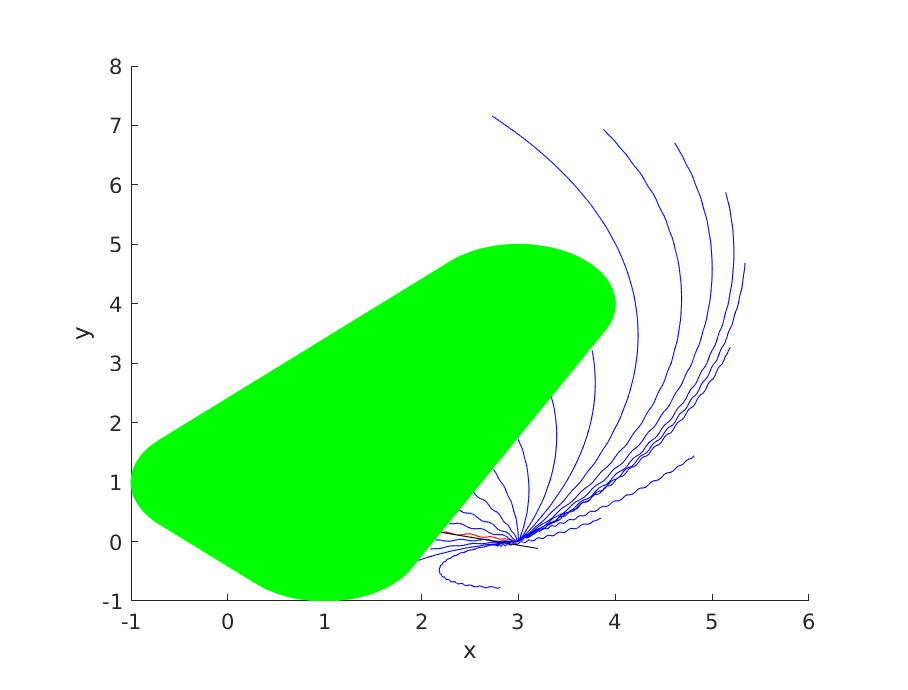
\includegraphics[width=0.7\textwidth]{pic_1.eps}\\
		{Рис. 1. Оптимальная траектория, $T = 0.1627$, $e_{right} = 0.0662$(погрешность $\psi) $}
	\end{center}
	
	\begin{center}	
		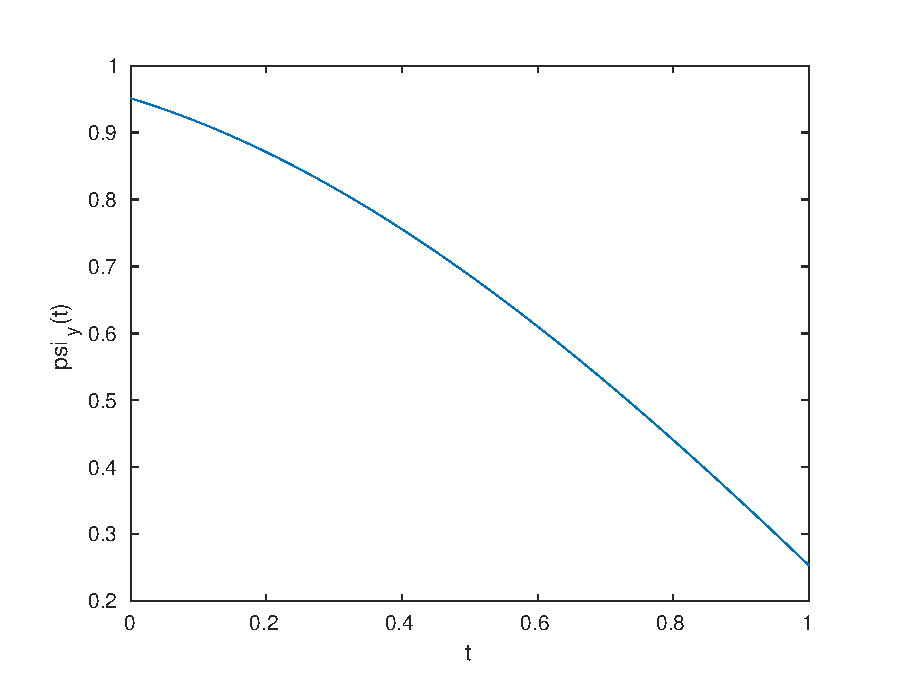
\includegraphics[width= 0.7	\textwidth ]{pic_2.eps}\\		
		{Рис. 2. Компонента $\psi_y(t)$ сопряженной системы}
	\end{center}
	
	\newpage
	
	\begin{center}
		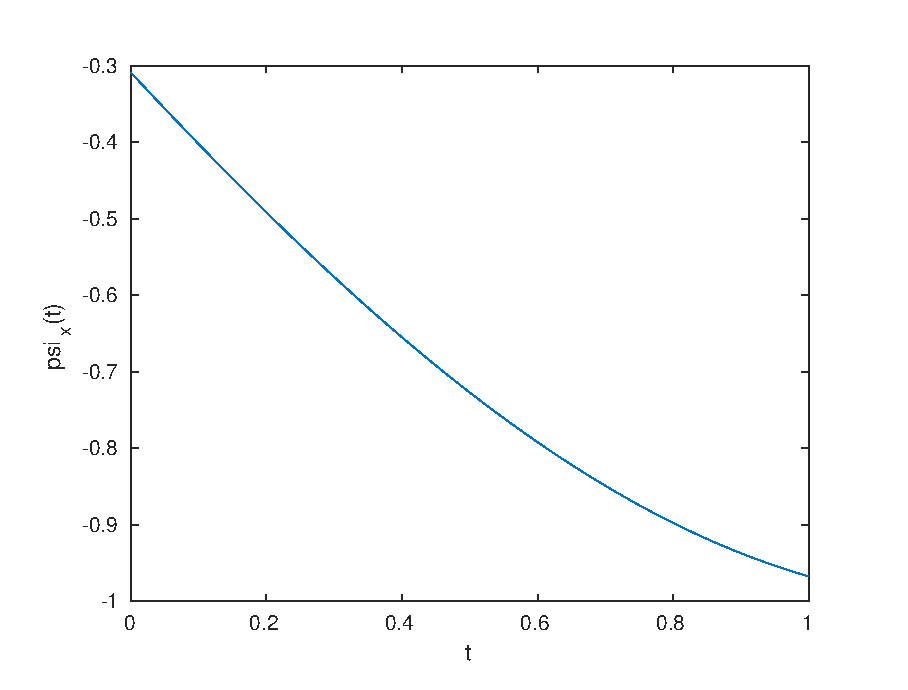
\includegraphics[width=0.7\textwidth]{pic_3.eps}\\
		{Рис. 3. Компонента $\psi_x(t)$ сопряженной системы}
	\end{center}
	\begin{center}	
		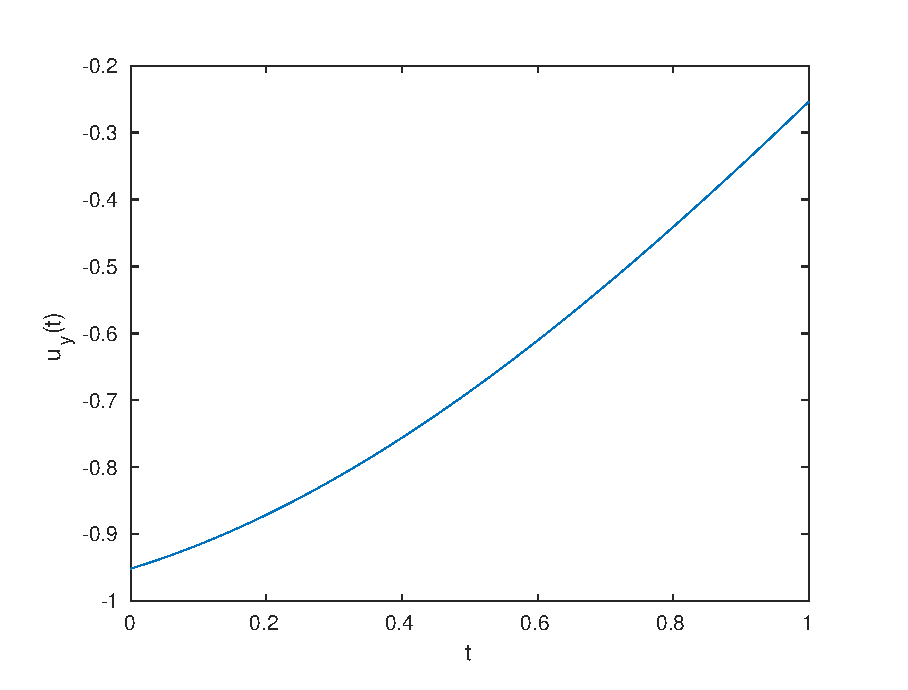
\includegraphics[width= 0.7\textwidth ]{pic_4.eps}\\		
		{Рис. 4. Компонента $u_y(t)$ оптимального управления}
	\end{center}

	\newpage

\begin{center}
	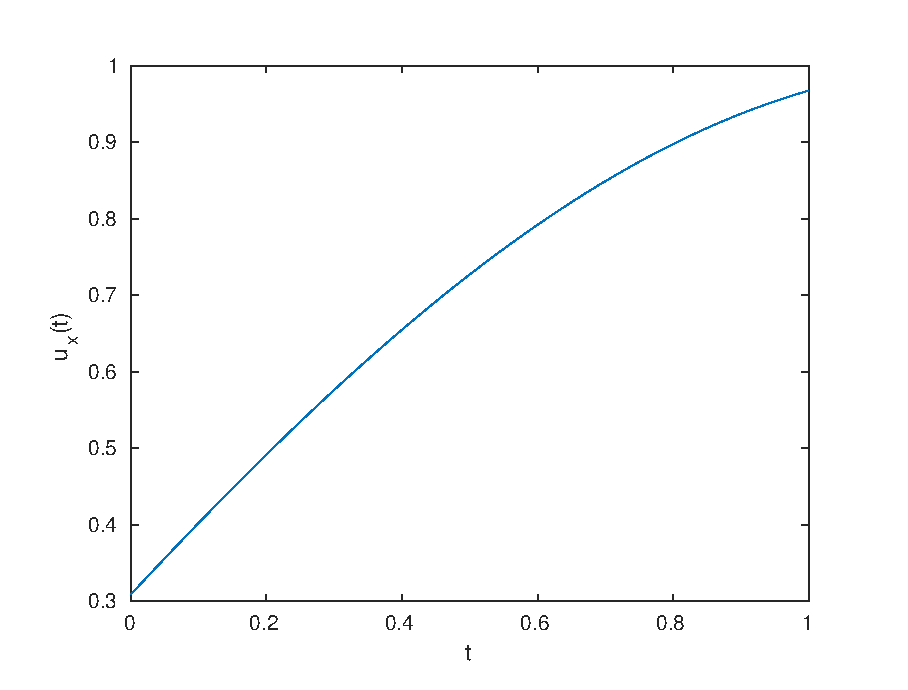
\includegraphics[width=0.7\textwidth]{pic_5.eps}\\
	{Рис. 5. Компонента $u_x(t)$ оптимального управления}
\end{center}
\begin{center}	
	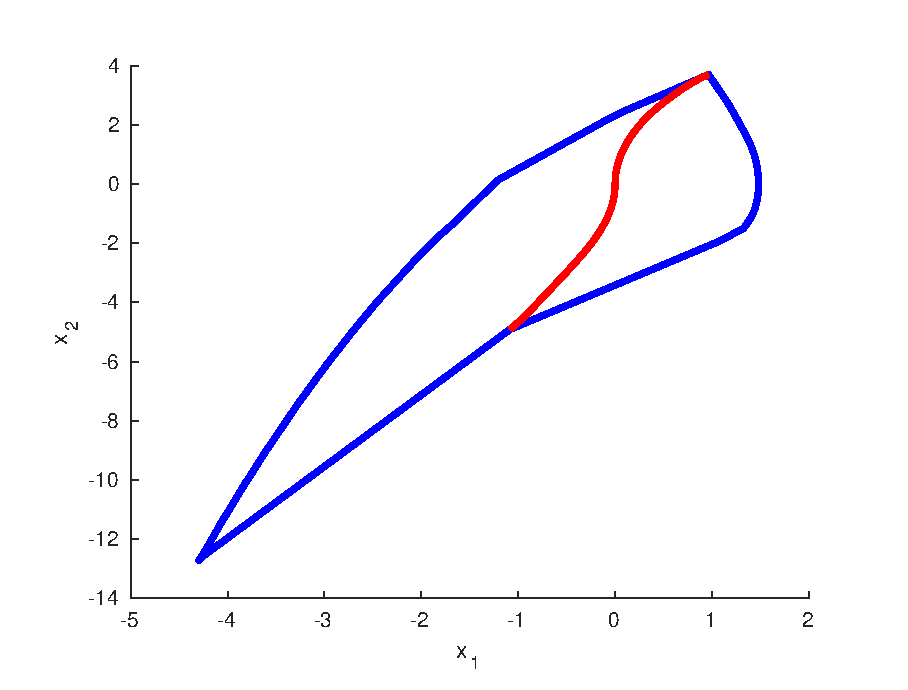
\includegraphics[width= 0.7\textwidth ]{pic_6.eps}\\		
	{Рис. 6. Компонента $y(t)$ оптимальной траектории}
\end{center}

	\newpage

\begin{center}
	\includegraphics[width=0.7\textwidth]{pic_7.eps}\\
	{Рис. 7. Компонента $x(t)$ оптимальной траектории}
\end{center}

\newpage

{\vspace*{-2cm} \hspace*{-1cm} \textbf{Пример 2}}
\[A = \begin{pmatrix}
3&0\\
0&-2
\end{pmatrix},
B = \begin{pmatrix}
-5&0\\
0&5
\end{pmatrix},
f = \begin{pmatrix}
0\\
0
\end{pmatrix} ,
x_1 = \begin{pmatrix}
1\\
1
\end{pmatrix},
q_1 = \begin{pmatrix}
0\\
3
\end{pmatrix},
q_2 = \begin{pmatrix}
-1\\
0
\end{pmatrix},
q_3 = \begin{pmatrix}
1\\
0
\end{pmatrix} \]
\[p_1 = 0, p_2 = 0, \alpha = 1,\beta = 1,\gamma = 1, r = 0. \]

\begin{center}
	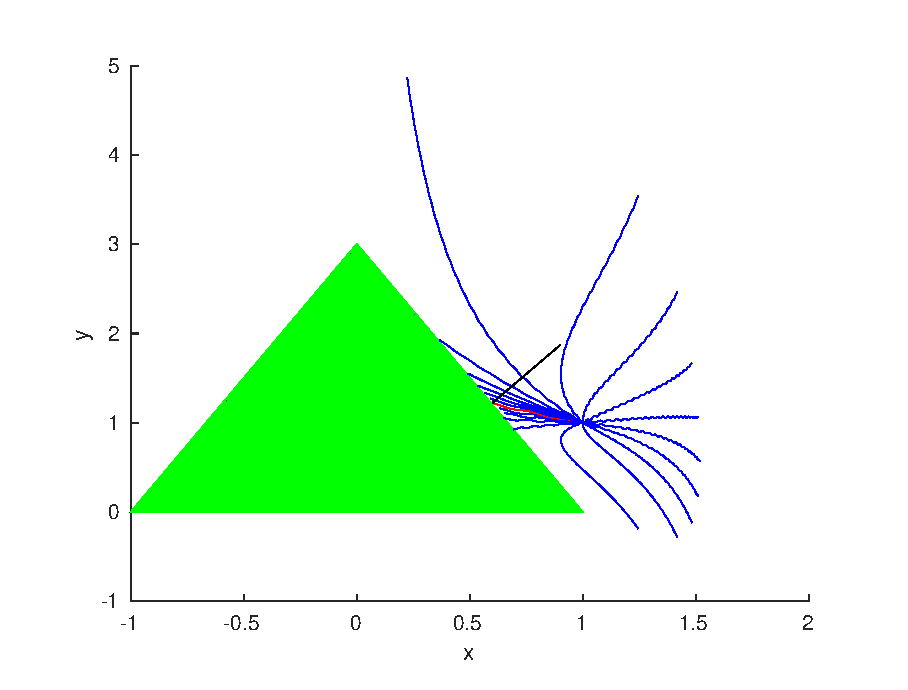
\includegraphics[width=0.7\textwidth]{pic_8.eps}\\
	{Рис. 8. Оптимальная траектория, $T = 0.0547,e_{right} = 0.5432$}
\end{center}

\begin{center}
	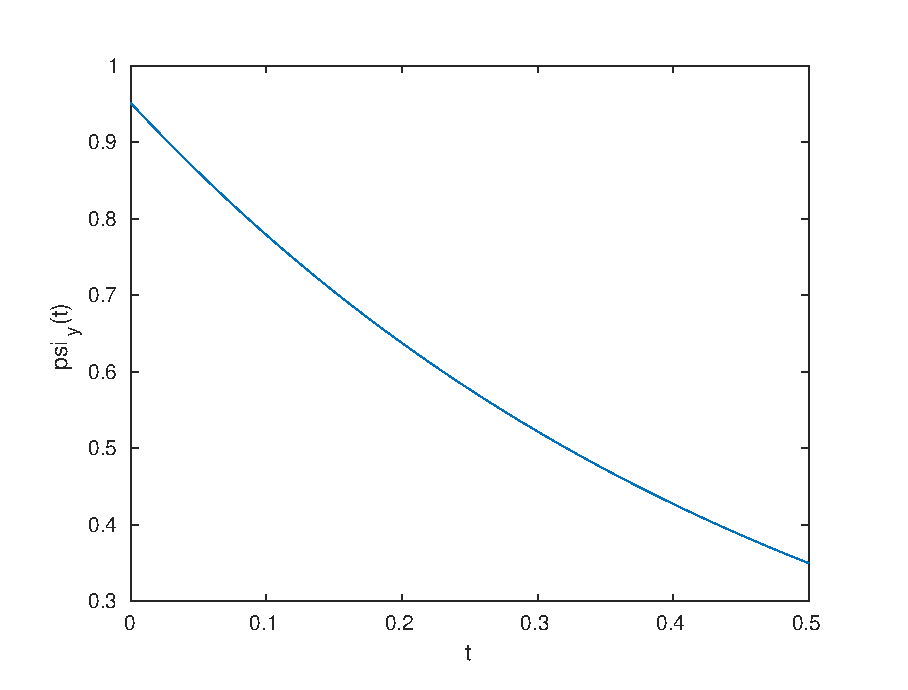
\includegraphics[width=0.7\textwidth]{pic_9.eps}\\
	{Рис. 9. Компонента $\psi_y(t)$ сопряженной системы}
\end{center}

\begin{center}
	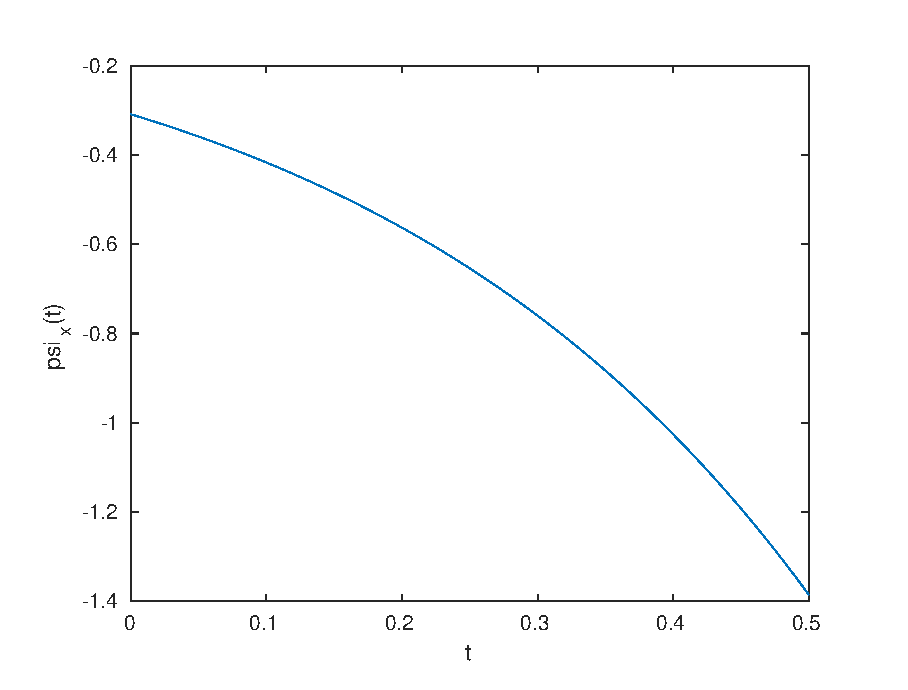
\includegraphics[width=0.7\textwidth]{pic_10.eps}\\
	{Рис. 10. Компонента $\psi_x(t)$ сопряженной системы}
\end{center}

\begin{center}
	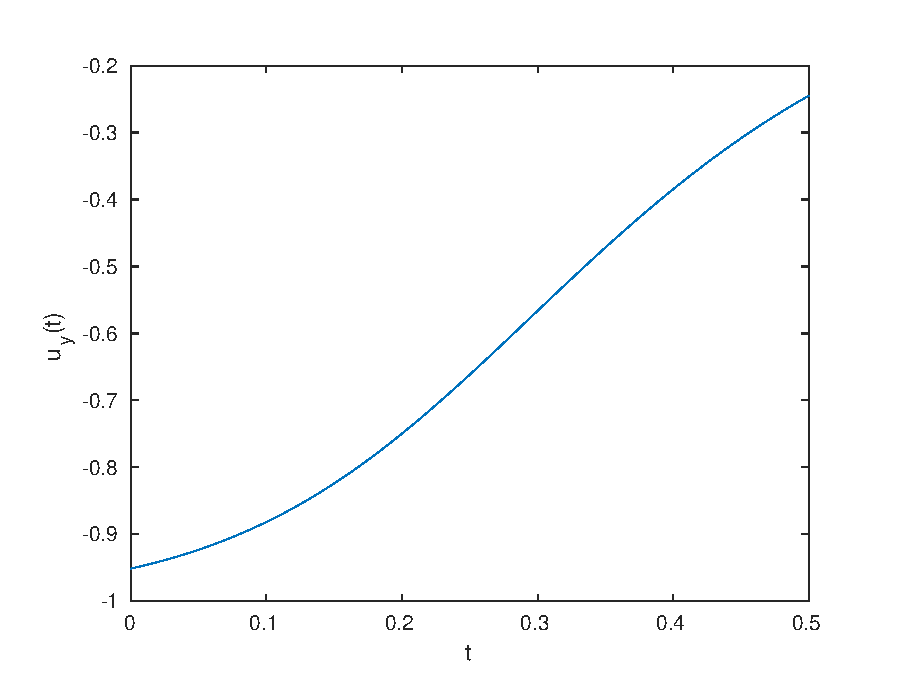
\includegraphics[width=0.7\textwidth]{pic_11.eps}\\
	{Рис. 11. Компонента $u_y(t)$ оптимального управления}
\end{center}

\begin{center}
	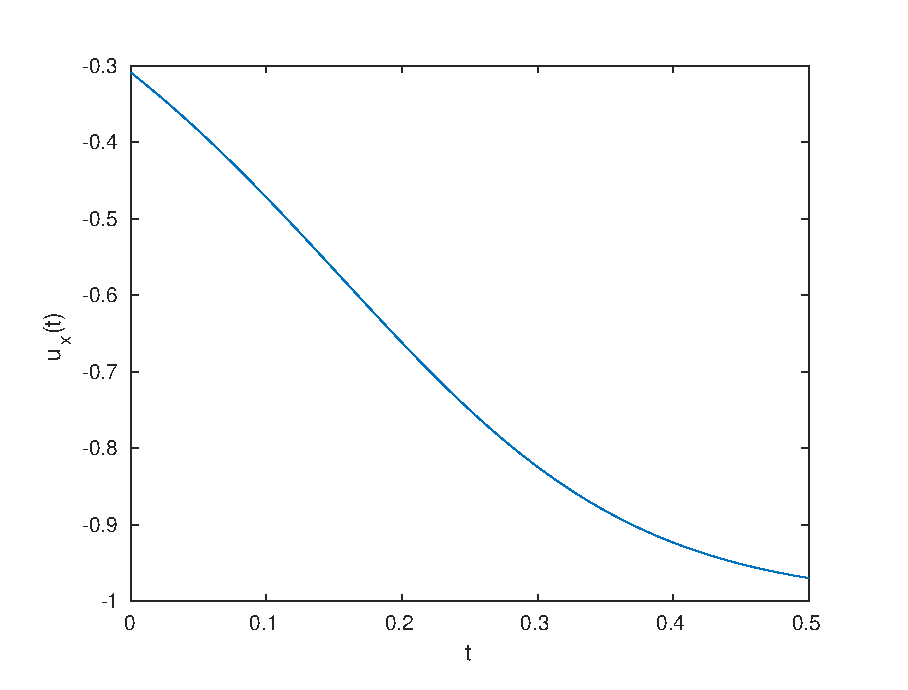
\includegraphics[width=0.7\textwidth]{pic_12.eps}\\
	{Рис. 12. Компонента $u_x(t)$ оптимального управления}
\end{center}

\begin{center}
	\includegraphics[width=0.7\textwidth]{pic_13.eps}\\
	{Рис. 13. Компонента $y(t)$ оптимальной траектории}
\end{center}

\begin{center}
	\includegraphics[width=0.7\textwidth]{pic_14.eps}\\
	{Рис. 14. Компонента $x(t)$ оптимальной траектории}
\end{center}

\newpage

{\vspace*{-2cm} \hspace*{-1cm} \textbf{Пример глобального улучшение результата задачи}}
\[A = \begin{pmatrix}
0&1\\
-1&0
\end{pmatrix},
B = \begin{pmatrix}
5&0\\
0&5
\end{pmatrix},
f = \begin{pmatrix}
2\\
-2
\end{pmatrix} ,
x_1 = \begin{pmatrix}
3\\
0
\end{pmatrix},
q_1 = \begin{pmatrix}
-10\\
3
\end{pmatrix},
q_2 = \begin{pmatrix}
-8\\
3
\end{pmatrix},
q_3 = \begin{pmatrix}
-5.6\\
-2.6
\end{pmatrix} \]
\[p_1 = 0, p_2 = 0, \alpha = 1,\beta = 1,\gamma = 1, r = 0.2, n = 15. \]
{Где $n$ --- это количество начальных условий для сопряженной системы(иными словами количество траекторий).}

\begin{center}
	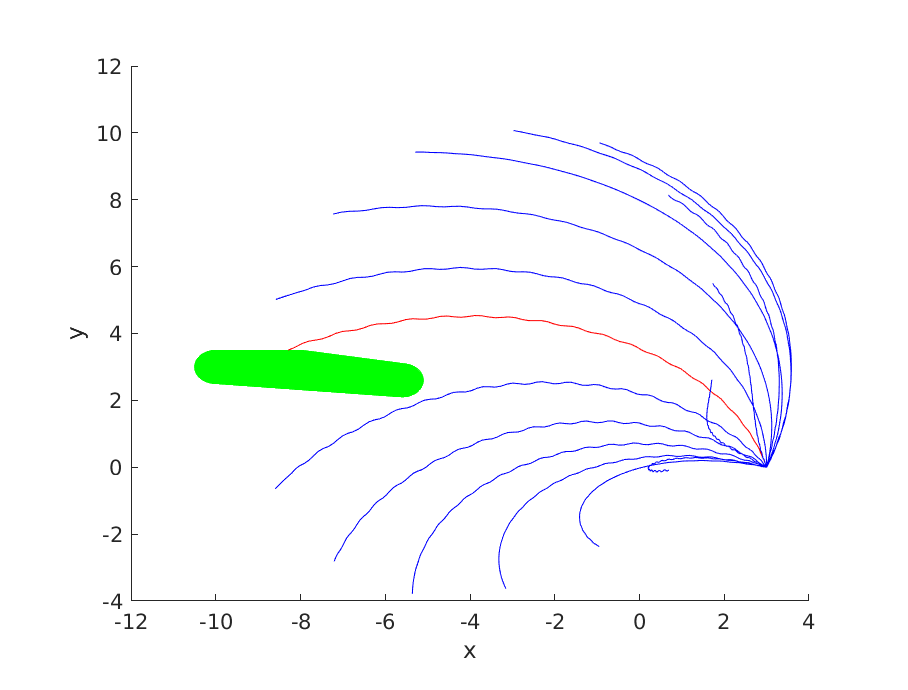
\includegraphics[width=0.7\textwidth]{pic_ulc_1.eps}\\
	{Рис. 15. Траектории при $n = 15$,$ \ T = 1.37912, e_{right} = 0.0900$}
\end{center}
{Увеличим количество начальных условий для сопряженной системы ($ n = 100$) и посмотрим на результат:}
\begin{center}
	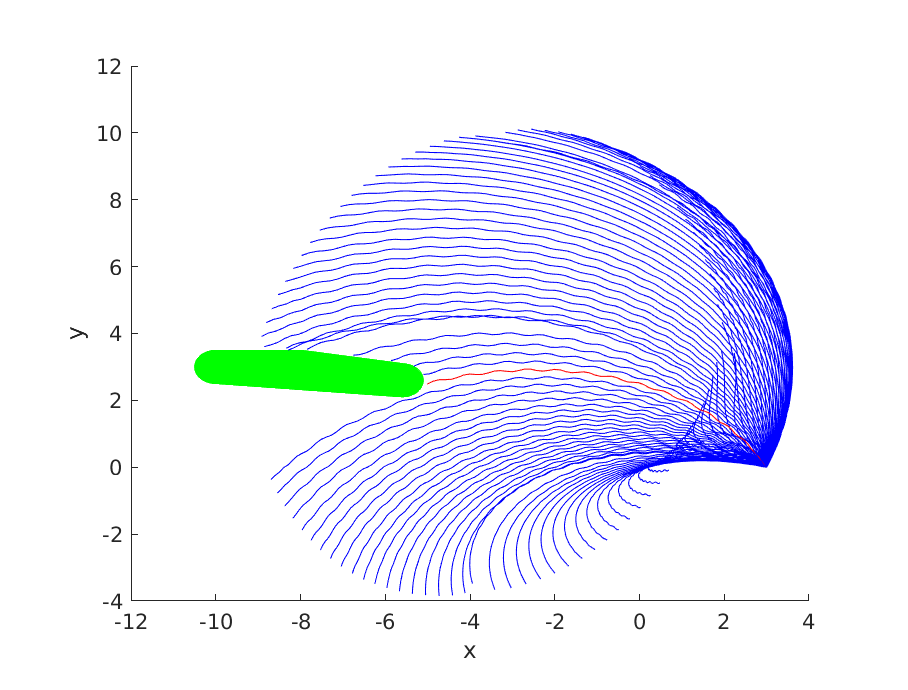
\includegraphics[width=0.7\textwidth]{pic_ulc_2.eps}\\
	{Рис. 16. Траектории при $n = 100$,$ \ T = 1.0582,e_{right} = 0.4563$}
\end{center}
{Как видно, в данном примере, в отличие от предыдущего, время сократилось.}
\newpage
{\vspace*{-3cm}\section{Исследование величины $T$ на непрерывность по начальному множеству фазовых переменных} }

\[A = \begin{pmatrix}
0&-1\\
1&0
\end{pmatrix},
B = \begin{pmatrix}
-5&0\\
0&-5
\end{pmatrix},
f = \begin{pmatrix}
-1\\
1
\end{pmatrix} ,
x_1 = \begin{pmatrix}
0.85\\
9
\end{pmatrix},
q_1 = \begin{pmatrix}
0\\
3
\end{pmatrix},
q_2 = \begin{pmatrix}
-1\\
0
\end{pmatrix},
q_3 = \begin{pmatrix}
1\\
0
\end{pmatrix} \]
\[p_1 = 0, p_2 = 0, \alpha = 1,\beta = 1,\gamma = 1, r = 0, t_{max} = 6. \]

\begin{center}
	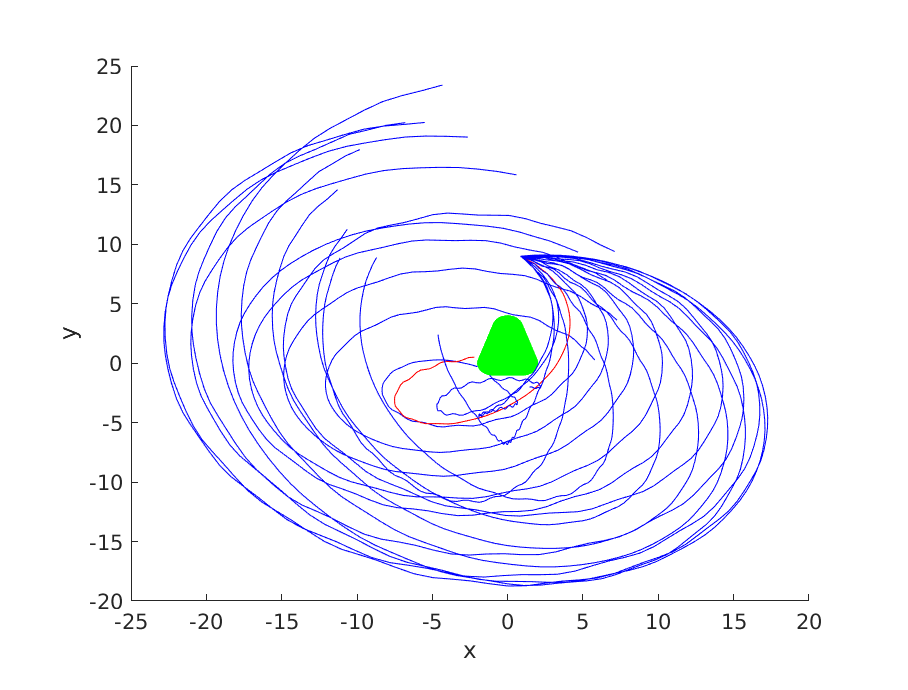
\includegraphics[width=0.7\textwidth]{pic_t_2.eps}\\
	{Рис. 17.\ Исходное множество. \ $T_1 = 4.5922$}
\end{center}
{Слегка сместим исходное множеств $\mathcal{X}_1$:}
\[ x_1 = \begin{bmatrix}
0.84\\
9
\end{bmatrix}. \]

\begin{center}
	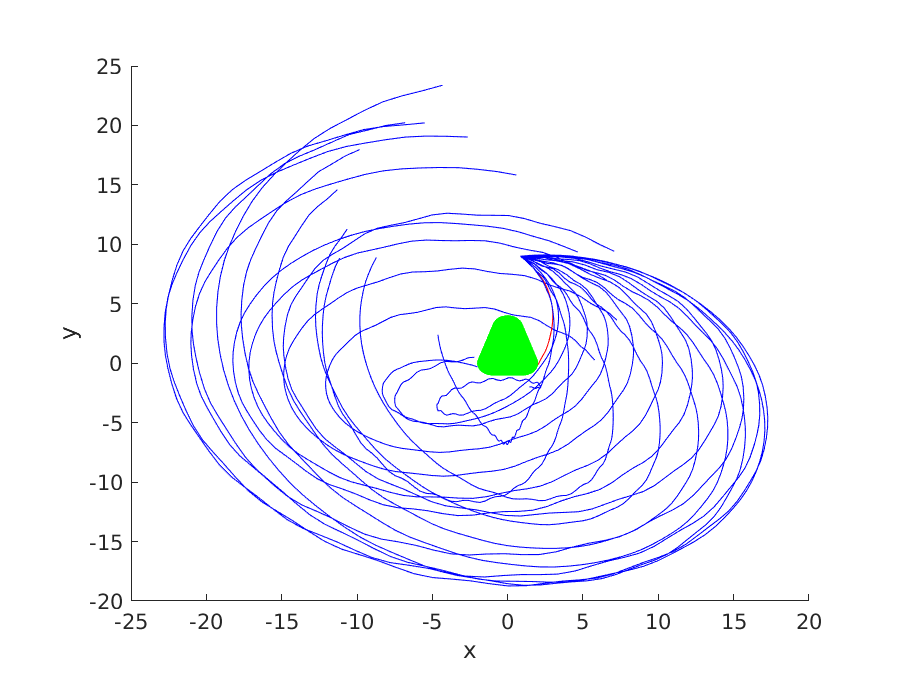
\includegraphics[width=0.7\textwidth]{pic_t_1.eps}\\
	{Рис. 18.\ Смещенное множество.  \ $T_1 = 1.3545$}
\end{center}
{Эти примеры подтверждают отсутствие непрерывности $T$.}
\newpage
{\section{Список литературы}}
{\hspace*{-0.6cm}[1] Комаров Юрий, лекции по оптимальному управлению. ВМК МГУ, Москва, 2020.}
\newline
\newline
{[2] Арутюнов Арам Владимирович, ''Лекции по выпуклому и многозначному анализу'', ВМК МГУ, Москва, 2020.}
\end{document}	
	